\section{Resolución de corto}
\begin{enumerate}
    \item Qué es monopolio de emisión monetaria:
        \begin{itemize}
            \item Es cuando solo un banco puede emitir moneda.
            \item El banco central justifica eso por el hecho de querer dar uniformidad monetaria.
        \end{itemize}
    \item Qué significa el banco central sea banquero del gobierno:
        \begin{itemize}
            \item Ellos financian al gobierno.
        \end{itemize}
    \item Cómo se relacionan la creación de bancos centrales en CA y la inflación del siglo XX: 
        \begin{itemize}
            \item La emisión de moneda causó inflación.
        \end{itemize}
\end{enumerate}

%%%%%%%%%%%%%%%%%%%%%%%%%%%%%%%%%%%%%%%%%%%%%%%%%%%%%%%%%%%%%%%%%%%%%%%%%%%%%%%%%%%%%%%%%%%%%%%%
\section{Noticia}
\begin{enumerate}
    \item Veblen goods
        \begin{itemize}
            \item Los bienes cuando se aprecian se tratan como nuevo bien porque empiezan a satisfacer necesidades diferentes.
            \item El problema de los bienes veblen, se valoran por la satisfacción que tienen la capacidad de derivar.
        \end{itemize}
\end{enumerate}

%%%%%%%%%%%%%%%%%%%%%%%%%%%%%%%%%%%%%%%%%%%%%%%%%%%%%%%%%%%%%%%%%%%%%%%%%%%%%%%%%%%%%%%%%%%%%%%%
\section{Discusión de clase}
\begin{enumerate}
    \item La rata comboyana:
        \begin{itemize}
            \item Los comunistas vienen y cometen genocidio y matan a la mayoría ya, resulta que toda la capacidad productiva se muere.
            \item Las ratas comboyana se aprecian? aumento la demanda pero no la apreciación. 
        \end{itemize}
    
    \item La renta incrementa la demanda de ciertos productos.
    \item En GT lo que pasa con las gaseosas, es un bien de status.
    \item El efecto sustitución:
        \begin{itemize}
            \item Cuando aumentan los precio relativos, la demanda baja.
            \item Bajan precios relativos del bien, la demanda sube.
        \end{itemize}
    
    \item \textbf{Nos preguntamos:} ¿Cuando suben los precios de todo en realidad podríamos decir que lo que estamos haciendo una disminución de renta?
        \begin{itemize}
            \item Si todos los precios se duplican es como cortar la renta a la mitad.
        \end{itemize}
    
    \item El bien gifen:
        \begin{itemize}
            \item El efecto renta es más fuerte que supera el efecto sustitución.
        \end{itemize}
    
    \item \begin{center}
        \begin{figure}[htbp]
            \centering
            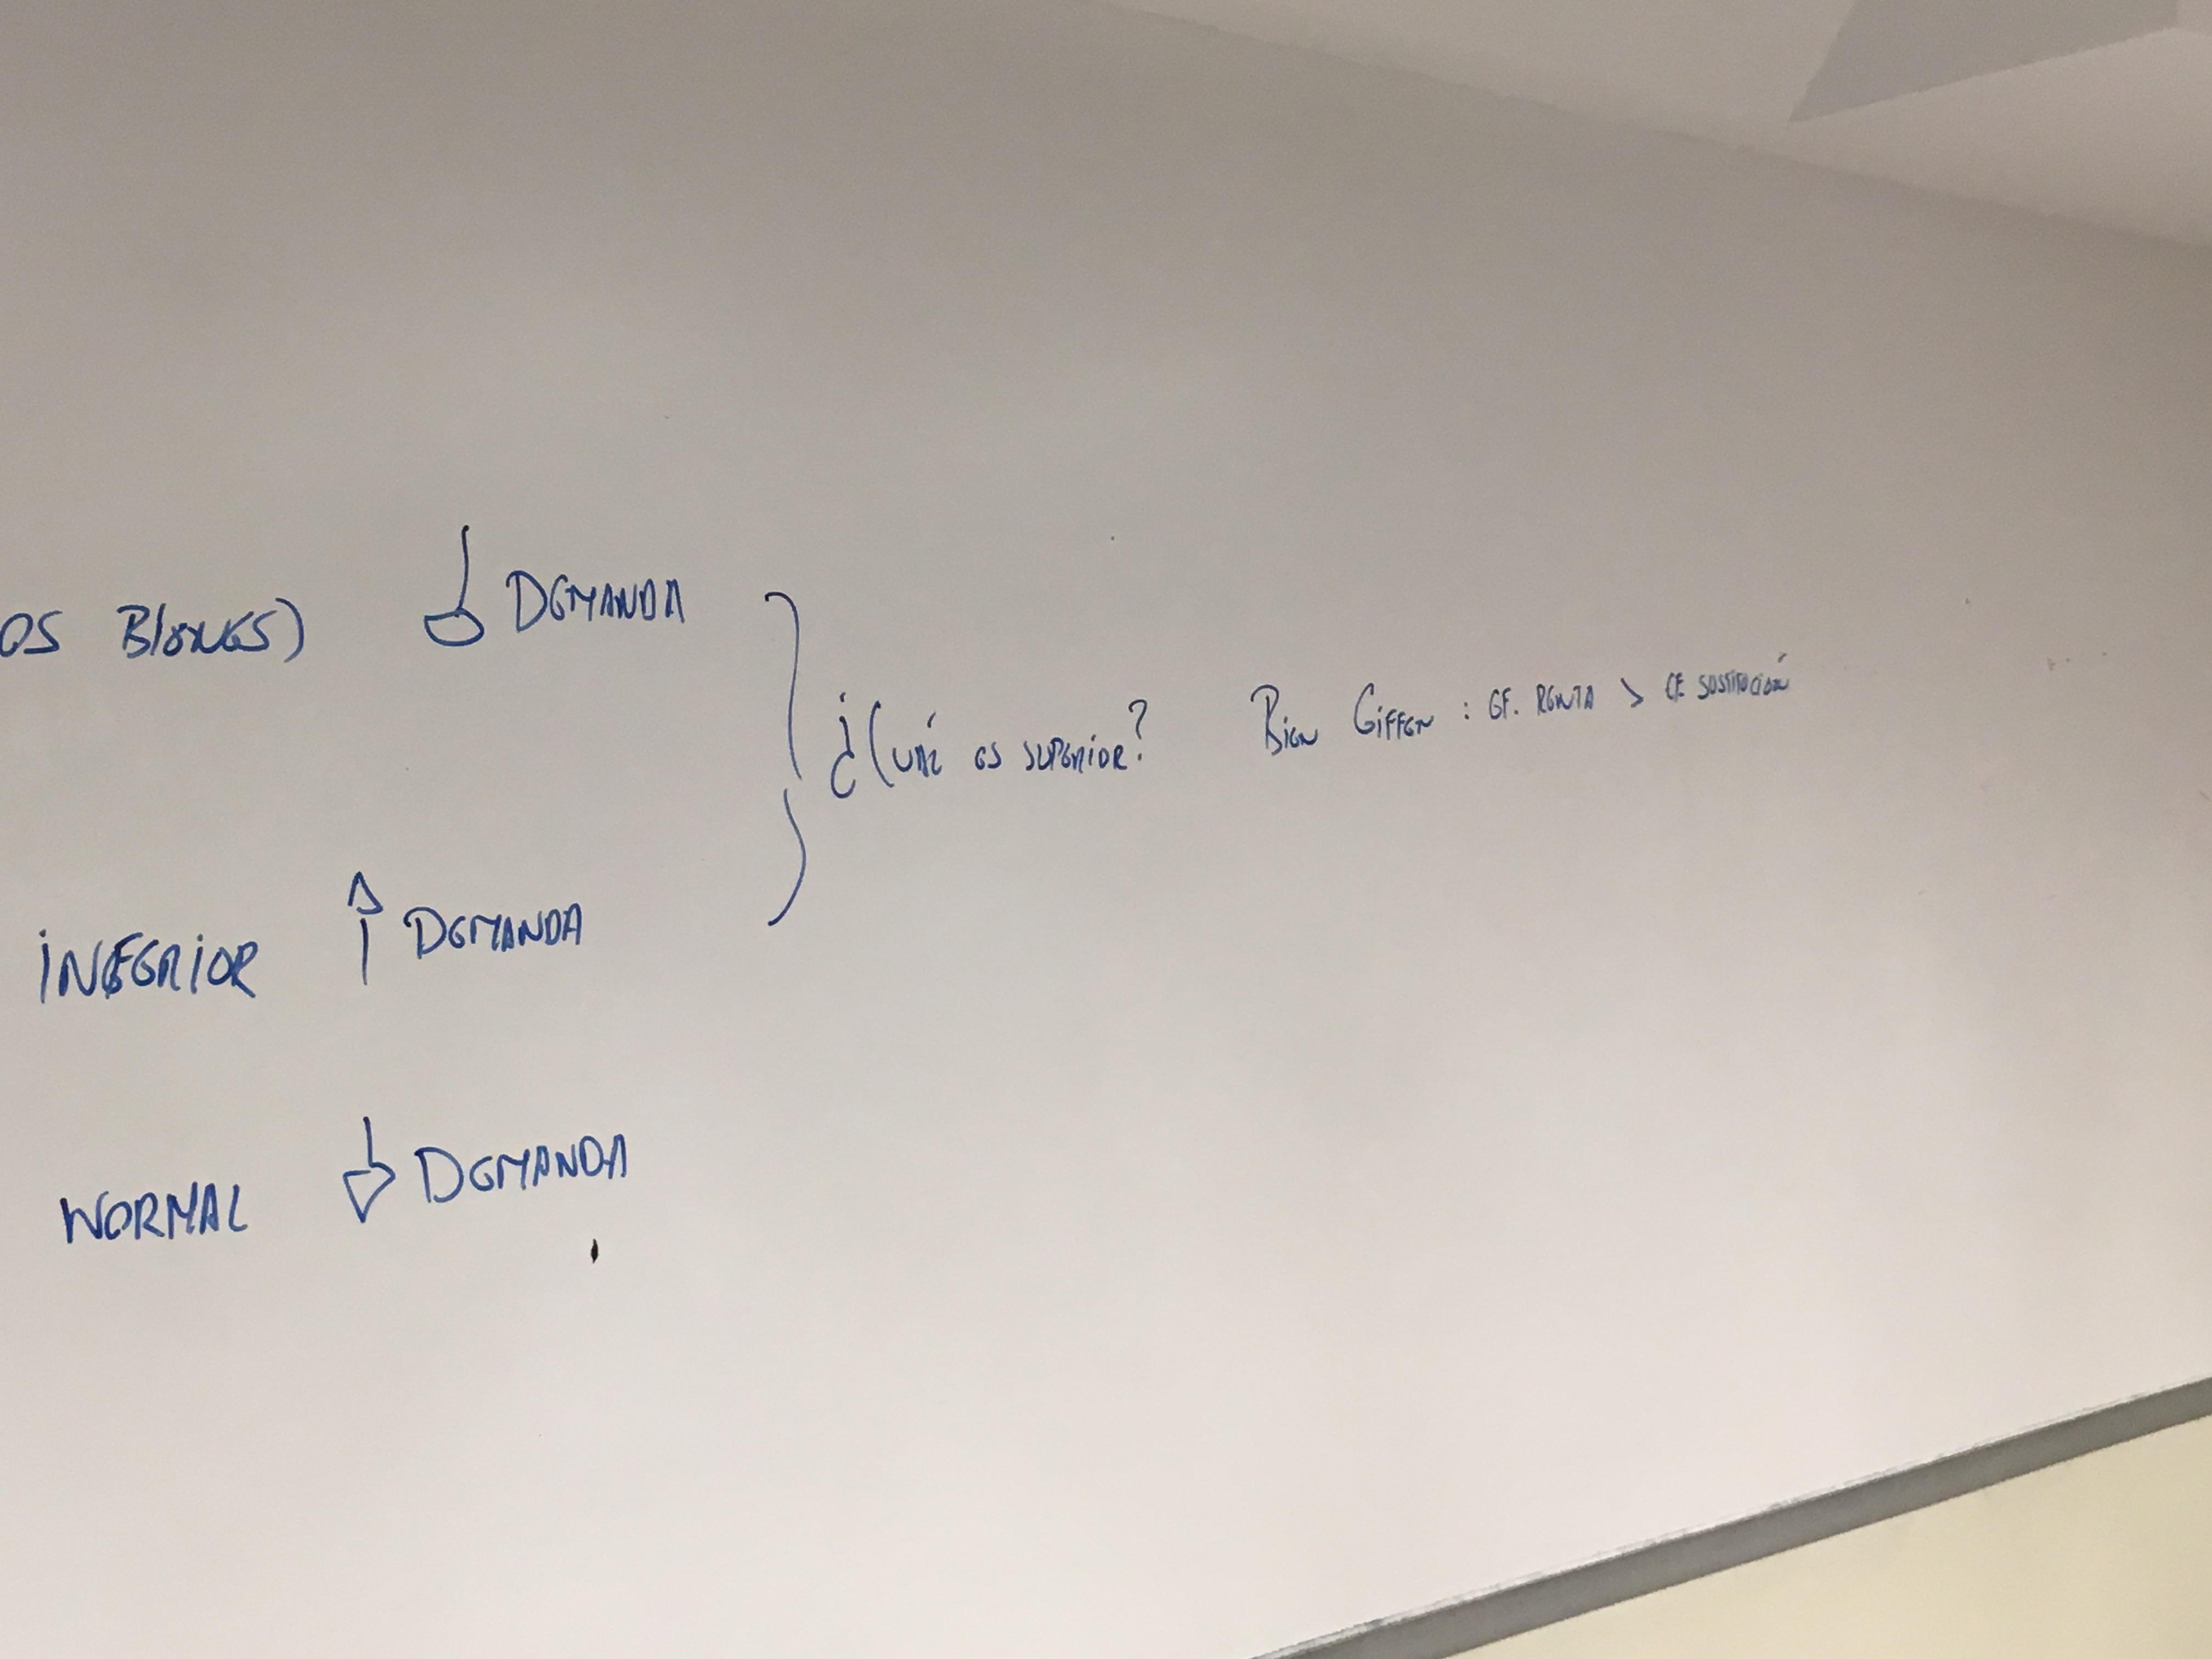
\includegraphics[width=9cm]{Classes/Images/photo-2.jpeg}
            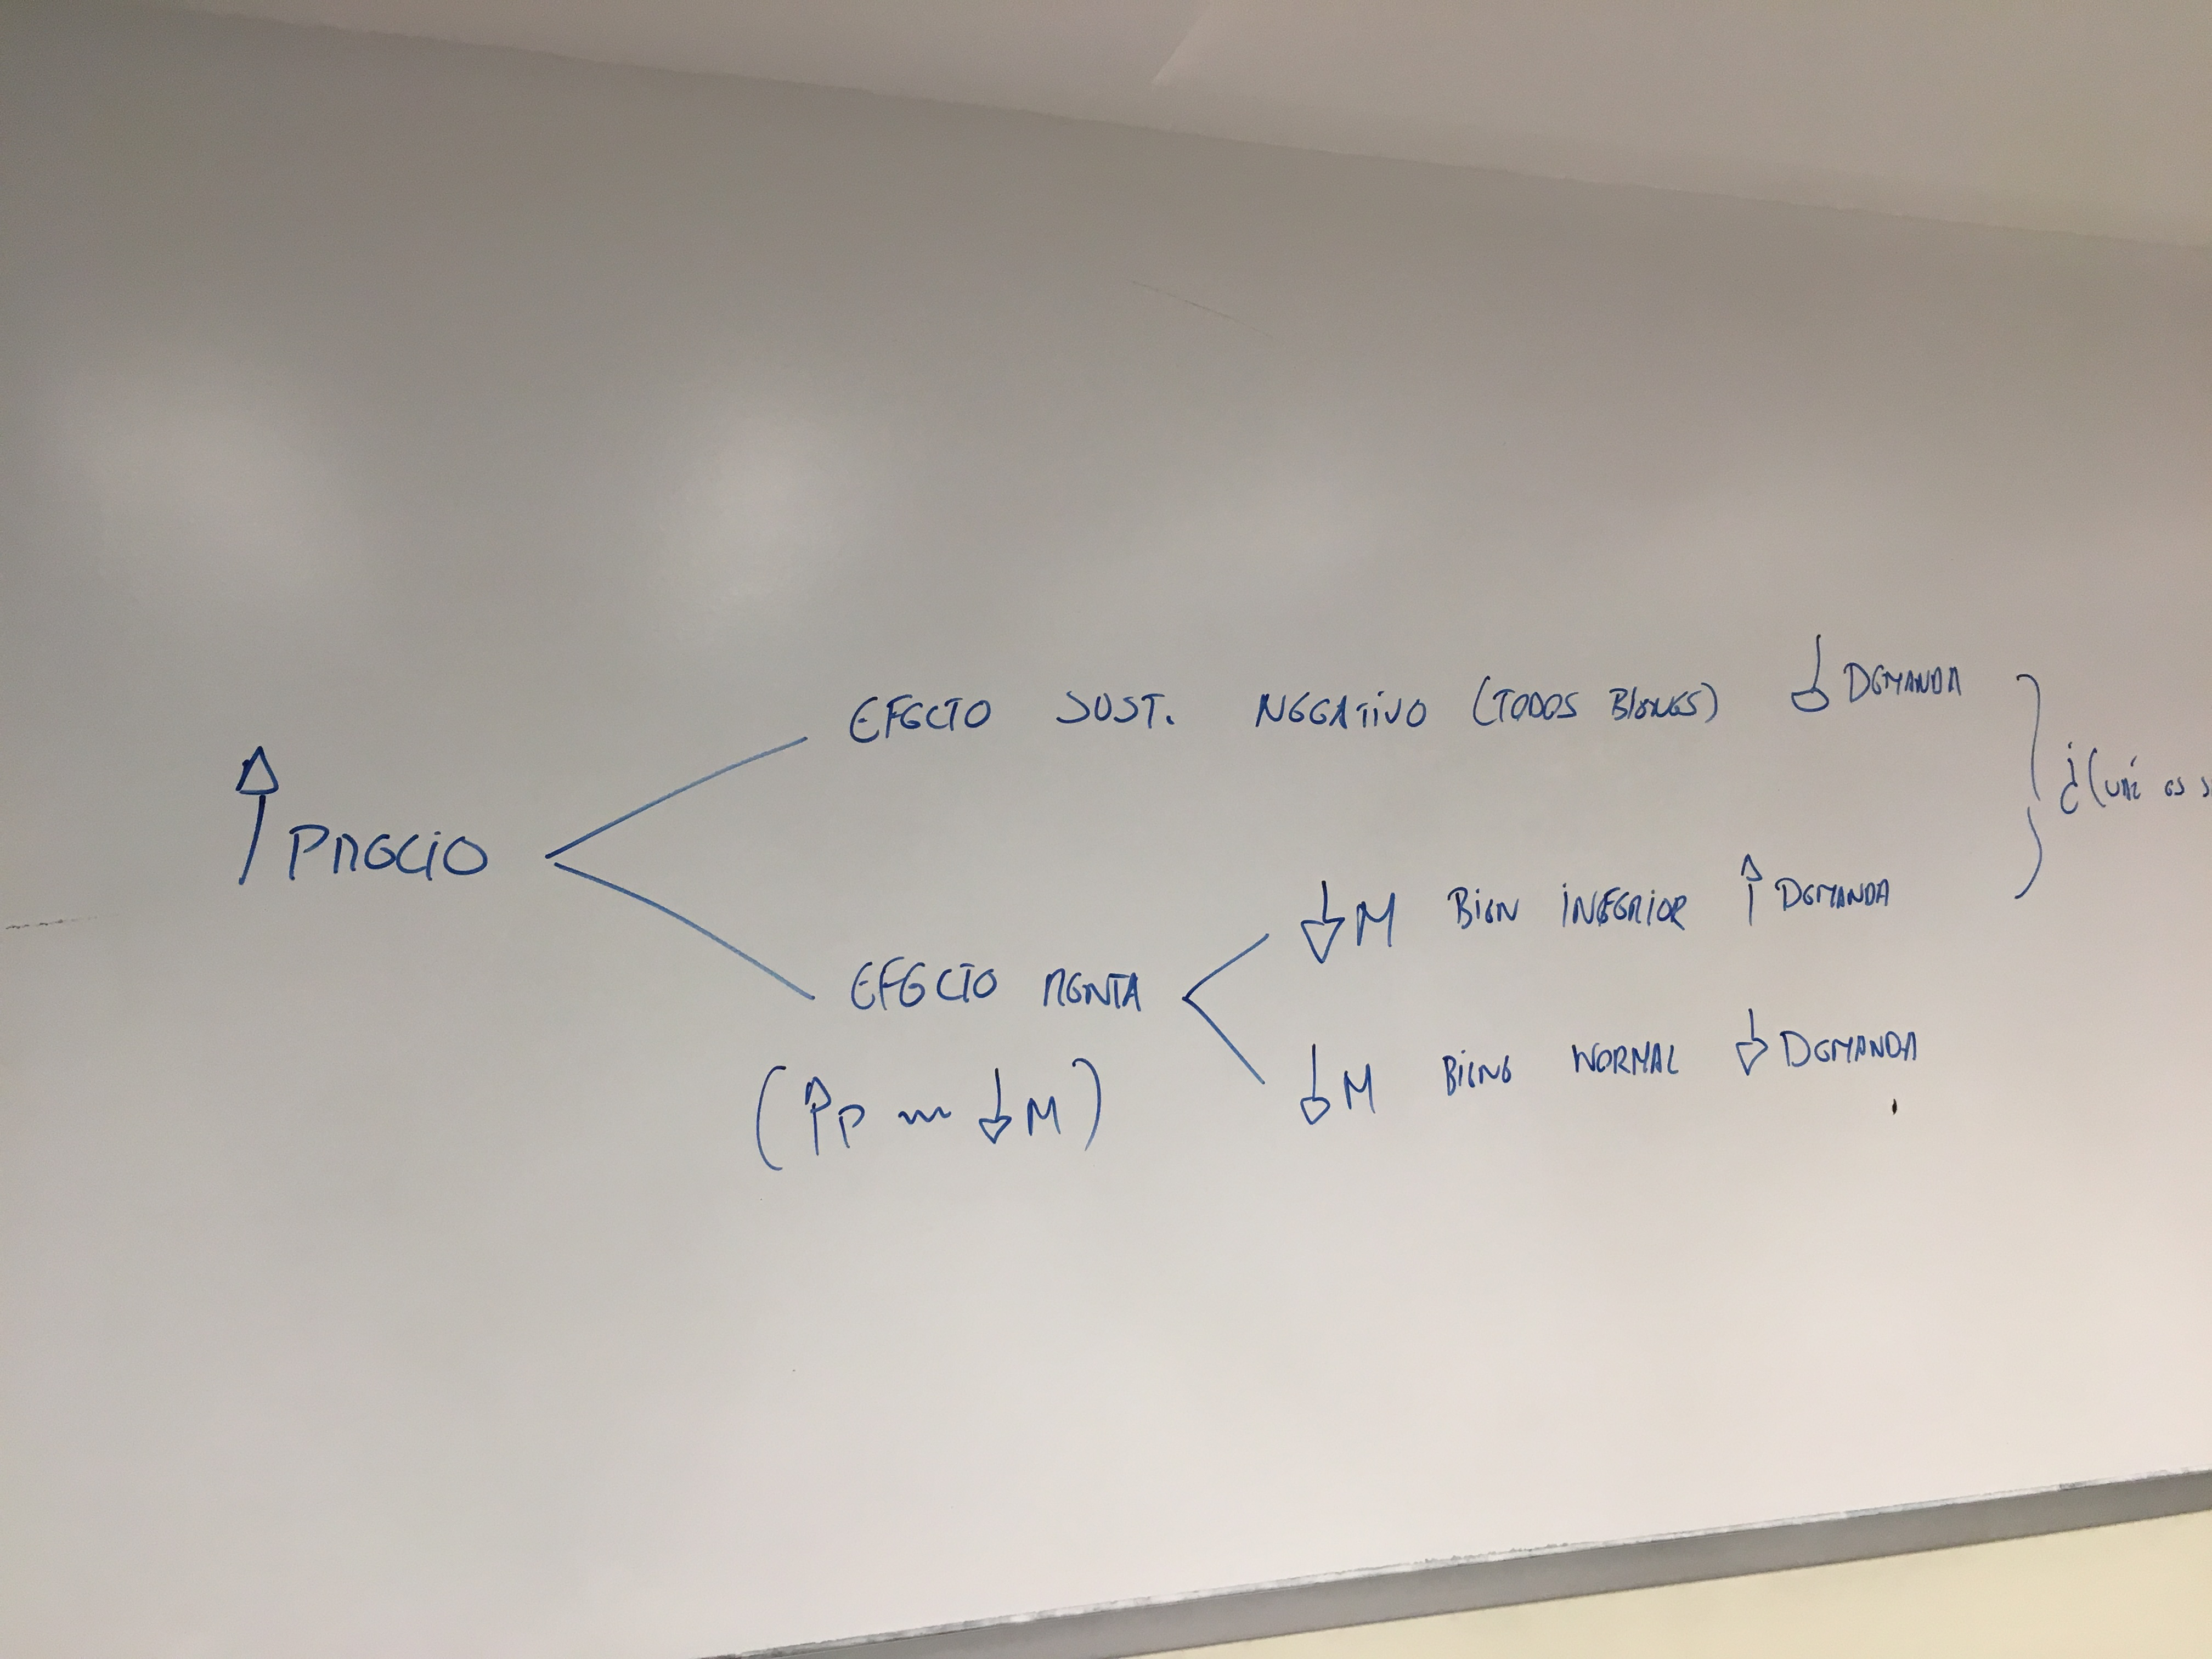
\includegraphics[width=9cm]{Classes/Images/photo.jpeg}
            \caption{}
            \label{}
        \end{figure}
    \end{center}
    
    \item Si los bienes en una economía se duplican los precios es $\equiv$ a una baja en la renta.
    \item El bien gifen es aquel cuyo efecto renta es superior al efecto sustitución.  
\end{enumerate}

%%%%%%%%%%%%%%%%%%%%%%%%%%%%%%%%%%%%%%%%%%%%%%%%%%%%%%%%%%%%%%%%%%%%%%%%%%%%%%%%%%%%%%%%%%%%%%%%
\section{Funciones de banca central}
\begin{enumerate}
    \item Reservas bancarias:
        \begin{itemize}
            \item Reservas bancarias: El banco central es el banco de bancos.
            \item El banco comercial deja sus reservas en el banco central, 
                \begin{itemize}
                    \item \emph{\textbf{Recordar lo siguiente: }los que circulan son los pagares.}
                    \item Los bancos centrales guardan el oro, ellos centralizan las reservas de oro, los bancos comerciales guardan un pequeña parte en sus bóvedas, y el resto lo dejan en el banco central.
                    \item El banco central le proporciona el mismo servicio a los bancos comerciales nos brindan a nosotros.
                    \item \textbf{Funciones legitimas}, los sistemas bancarios que no tenían una banca central tenían algo similar a un banco central ``privados'', \emph{\textbf{Ejemplo: }Los bancos de NY era la banca central privada antes de la reserva federal.}
                \end{itemize}
        \end{itemize}
    
    
    \item Cámara de compensación:
        \begin{itemize}
            \item El banco central es un facilitador de transacciones.
            \item El banco central es un banco de bancos, es una transacción de promesas.
            \item \emph{\textbf{Ejemplo: }Alguien paga a otra persona con cheque.}
            \item Los bancos comerciales tienen cuenta en el banco central y cuando un banco  
            \item Los bancos centrales sólo hacen las transferencias del diferencial al final del día.
        \end{itemize}
    
    \item Mantener estabilidad de precios:
        \begin{itemize}
            \item El objetivo más explicito.
            \item Los bancos centrales han aprendido.
            \item El banco central no tiene competencia, entonces que le hace cuidar el valor de sus monedas.
            \item En GT se está castigando la utilización de dólares.
            \item La competencia y la convertibilidad las dos son infalibles.
        \end{itemize}
    
    \item Estabilizar ciclos económicos y financieros:
        \begin{itemize}
            \item Cuando el sistema financiero tiene problemas o está con estrés.
            \item El estrés en el sistema financiero son corridas bancarias (todo el mundo va a sacar su dinero), cuando el banco se muestra incapaz de poder pagarle a sus clientes.
            \item En casos de estrés extremo el banco central son \textbf{prestamistas de última instancia}. 
            \item Los bancos centrales solo dan línea de crédito a bancos que están solventes.
            \item El banco comercial en estrés entregan como colateral los prestamos aceptados (que si paguen), el banco central abre una línea de crédito, entonces el banco comercial intercambia sus prestamos por liquidez.
            \item El banco central es el padre de toda la liquidez del sistema, puede darla toda sin perderla.
            \item \emph{\textbf{Consultar el siguiente recurso:}regla de Ragghot, regla de Horton}
            \item La función en suma es que los bancos van a tener corridas bancarias y el banco central tras evaluar la situación, presta y salva a dicho banco.
            \item Estas cosas es por a cual no tenemos patrón oro.
        \end{itemize}
    
    \item \emph{\textbf{(Paréntesis ``Riesgo moral'':} lo que pasa es que los bancos están haciendo barbaridades por que saben que el banco central los va a ganar, esto es lo que se llama crony capitalism (privatizar la ganancia y socializar las pérdidas) entonces los bancos son incentivados a hacer lo que quieran por que la banca central los salva, por esto es que el moral hazard es un problema muy malo, por esto dejaron quebrar Leman Brothers y no a los demás. El banco central tiene un tipo de interés alto por el hecho de tener que dar un incentivo a no acudir al banco central para adquirir ganancia.}
        \begin{itemize}
            \item El gobierno no puede impedir la imprudencia.
            \item Puede incentivar a no ser imprudente.
        \end{itemize}
\end{enumerate}
